\chapter[Misure e osservabili]{Misure, osservabili e principio di indeterminazione\footnote{S1.4}}
Discutiamo qui la \textbf{teoria quantistica della misura}. In meccanica quantistica, per un sistema che si trovi in un determinato stato iniziale $\vert \varphi \rangle$, una misura di una quantità fisica non produce,in generale, sempre lo stesso risultato. Piuttosto si possono ottenere differenti risultati, ciascuno con una determinata probabilità.\\
Se indichiamo con $a_i$ i possibili risultati di una misura dell'osservabile $A$ e con $P_i$ le relative probabilità (riferite ad un sistema che si trovi nello stato $\vert \varphi \rangle$) possiamo scrivere il \textbf{valore medio} dei risultati di una misura $A$ come
\begin{equation}
\langle A \rangle = \sum _i a_i P_i.
\end{equation}
\textbf{Nella meccanica quantistica si associa ad ogni grandezza fisica $A$ un operatore lineare che la rappresenta:}

\begin{equation}
\begin{array}{c}
\textrm{Grandezza fisica}\\
A
\end{array}
\longleftrightarrow
\begin{array}{c}
\textrm{Operatore}\\
A
\end{array}
\end{equation}
\textbf{L'operatore $A$ viene definito in maniera tale che, per un sistema che si trovi in uno stato $\vert \varphi \rangle $, valga la relazione}
\begin{equation}
\langle A \rangle = \langle \varphi \vert A \vert \varphi \rangle,
\end{equation}
ossia il valor medio dei possibili risultati di una misura di $A$ è dato dal \textbf{valore di aspettazione} dell'operatore $A$ sullo stato $\vert \varphi \rangle$.\\
naturalmente \textbf{i valori medi di qualsiasi grandezza fisica reale, in qualunque stato, sono reali}. Questa circostanza pone determinate limitazioni alle proprietà degli operatori che corrispondono, nella meccanica quantistica, alle grandezze fisiche. Assumiamo infatti che $\langle \varphi \vert A \vert \varphi \rangle$ sia reale per qualunque scelta del vettore di stato $\vert \varphi \rangle$. Consideriamo poi un vettore $\vert \varphi \rangle$ della forma
\begin{equation}
\vert \varphi \rangle = \alpha \vert u \rangle + \beta \vert v \rangle,
\end{equation}
dove $\alpha$ e $\beta$ sono numeri complessi. Il valore di aspettazione di $A$ su questo stato è dato da:
\begin{eqnarray}
& &\left( \alpha ^* \langle u \vert + \beta ^* \langle v \vert \right) A \left(\alpha \vert u \rangle + \beta \vert v \rangle \right) = \nonumber \\
& &=\vert \alpha \vert ^2 \langle u \vert A \vert u \rangle + \vert \beta \vert ^2 \langle v \vert A \vert v \rangle + \alpha ^* \beta \langle u \vert A \vert v \rangle \alpha  \beta ^* \langle v \vert A \vert u \rangle
\end{eqnarray}
Per ipotesi, i primi due termini che entrano in questa espressione sono reali. Deve dunque essere reale anche la somma dei due secondi termini. Uguagliando la parte immaginaria di questa somma a zero otteniamo:
\begin{equation}
\label{eq:cap4_1}
\alpha ^* \beta \left(\langle u \vert A \vert v \rangle -\langle u \vert A^{+} \vert v \rangle \right)-  \alpha  \beta ^* \left( \langle v \vert A^{+} \vert u \rangle -\langle v \vert A \vert u \rangle \right) =0, 
\end{equation}
da cui segue:
\begin{equation}
\langle u \vert A \vert v \rangle = \langle u \vert A^{+} \vert v \rangle ,
\end{equation}
Ma poiché i vettori $\vert u \rangle$ e $\vert v \rangle$ sono arbitrari concludiamo che
\begin{equation}
A= A^{+},
\end{equation}
ossia \textbf{gli operatori che rappresentano le osservabili in meccanica quantistica sono operatori hermitiani}.\\
(Viceversa se $A= A^{+}$ allora $\langle \varphi \vert A \vert \varphi \rangle$ è reale per definizione di $A^{+}$).\\ \\
la condizione (\ref{eq:cap4_1}) può essere scritta anche nella forma
\begin{equation}
\alpha ^* \beta m - \left( \alpha ^*  \beta \right) ^* m^* =0, 
\end{equation}
dove $m= \left( \langle u \vert A \vert v \rangle - \langle u \vert A^{+} \vert v \rangle \right)$. Scegliendo allora $\alpha ^* \beta$ reale oppure $\alpha ^* \beta$ immaginario puro si ottiene rispettivamente
\begin{equation}
\begin{cases}
\alpha ^* \beta \left( m- m^* \right) =0 \\
\alpha ^* \beta \left( m + m^* \right) =0
\end{cases}
\Rightarrow
\begin{cases}
m= m^*\\
m= - m^*
\end{cases}
\end{equation}
che implicano necessariamente
\begin{equation}
m=0.
\end{equation}
\section{Autovalori ed autovettori di osservabili}
Cerchiamo di determinare i possibili valori della grandezza $A$ e gli stati $\vert a' \rangle$ nei quali tale grandezza non può avere che un solo valore determinato $a'$. Per tali stati lo \textbf{scarto quadratico medio} 
\begin{equation}
\langle \left( \Delta A \right) ^2 \rangle \equiv \langle \left( A- \langle A\rangle \right) ^2 \rangle
\end{equation}
deve essere nullo.\\
Calcoliamo allora esplicitamente il valore di aspettazione di $(\Delta A )^2$ sullo stato $\vert a' \rangle$, ponendo dunque $\langle A \rangle = a'$. Utilizzando la relazione di completezza per un insieme arbitrario di stati di base si ottiene:
\begin{eqnarray}
0 & = & \langle a' \vert (\Delta A )^2 \vert a'\rangle = \langle a' \vert (A-a' )(A-a') \vert a'\rangle= \nonumber \\
& = & \sum _i \langle a' \vert (A-a' ) \vert i \rangle \langle i \vert (A-a' ) \vert a' \rangle = \\
& = & \sum _i \langle i \vert (A^{+}-a' ) \vert a' \rangle ^* \langle i \vert (A-a' ) \vert a' \rangle = \nonumber \\
& = & \sum _i \vert \langle i \vert (A-a' ) \vert a' \rangle \vert ^2.\nonumber
\end{eqnarray}
Poiché ciascun termine della sommatoria è positivo o nullo, questa condizione può essere soddisfatta solo se
\begin{equation}
\langle i \vert A-a' \vert a' \rangle =0 \qquad \textrm{ per ogni } \vert i \rangle .
\end{equation}
Otteniamo quindi la relazione
\begin{equation}
A \vert a' \rangle =a' \vert a' \rangle .
\end{equation}
Questa equazione è detta \textbf{equazione agli autovalori}. i numeri $a'$ sono detti \textbf{autovalori} dell'operatore $A$ ed i corrispondenti stati $\vert a' \rangle $ prendono il nome di \textbf{autostati od autovettori} dell'operatore.\\
Abbiamo così mostrato che \textbf{se un sistema si trova in uno stato corrispondente ad un autostato dell'operatore $A$ con autovalore $a'$, allora una misure dell'osservabile $A$ produce con certezza il valore $a'$. Viceversa, se una misura dell'osservabile $A$ in un determinato stato produce con certezza il valore $a'$, allora lo stato in questione è un autostato di $A$ corrispondente all'autovalore $a'$.}\\
\textbf{In meccanica quantistica si postula inoltre che la totalità degli autovalori dell'operatore $A$ è identica alla totalità di tutti i possibili risultati di una misura della grandezza $A$ corrispondente.}\\
È utile sottolineare la \textbf{distinzione tra autovalori e valori di aspettazione.} Per esempio, per una particella di spin $1/2$, i risultai di una misura della componente $z$ dello spin possono assumere solo i valori $\pm \hbar/2$ (corrispondenti agli autovalori dell'operatore $S_z$) mentre il valore di aspettazione di $S_z$ in un determinato stato può assumere in generale qualunque valore compreso tra $-\hbar /2$ e $+\hbar /2$.
\newpage
\section{Autovettori di osservabili come vettori di base}
Consideriamo due \textbf{proprietà degli operatori hermitiani:}
\begin{enumerate}
\item \textbf{Gli autovalori di un operatore hermitiano sono reali.} Indichiamo con $a'$ un autovalore di $A$ e con $\vert a' \rangle $ il corrispondente autovettore convenientemente normalizzato$\langle a' \vert a' \rangle =1 $. Possiamo allora scrivere
\begin{equation}
\langle a' \vert A \vert a' \rangle = a' \langle a' \vert a' \rangle = a'.
\end{equation}
D'altra parte, per l'hermitianità dell'operatore $A$ si ha pure
\begin{equation}
\langle a' \vert A \vert a' \rangle = \langle a' \vert A \vert a' \rangle  ^* = a'^*,
\end{equation}
da cui segue
\begin{equation}
a'=a'^* .
\end{equation}
Questo risultato è consistente con l'assunzione che gli autovalori di un operatore hermitiano $A$ rappresentano i possibili risultati di una misura della grandezza fisica reale $A$.
\item \textbf{Gli autovettori di un operatore hermitiano corrispondenti ad autovalori distinti sono ortogonali.}\\
indichiamo con $a' $ e $a''$ due autovalori distinti di $A$ e con $\vert a' \rangle$ ed $\vert a'' \rangle$ i corrispondenti autovettori. Si ha:
\begin{eqnarray}
\langle a' \vert A \vert a'' \rangle & = & a'' \langle a' \vert a'' \rangle  \nonumber \\
\\
\langle a' \vert A \vert a'' \rangle & = & \langle a'' \vert A \vert a' \rangle ^* = a' \langle a'' \vert a' \rangle ^* = a' \langle a' \vert a'' \rangle , \nonumber 
\end{eqnarray}
dove nella seconda equazione si è utilizzato il risultato secondo cui gli autovalori di un operatore hermitiano sono reali. Sottraendo allora membro a membro le due equazioni si ottiene
\begin{equation}
(a'-a'') \langle a' \vert a'' \rangle =0,
\end{equation}
ossia
\begin{equation}
\langle a' \vert a'' \rangle =0 \qquad \textrm{ per } a' \neq a'' .
\end{equation}
\end{enumerate}
Osserviamo che \textbf{in generale gli autostati associati ad uno stesso autovalore non sono ortogonali.} Poiché però una qualunque combinazione lineare di autostati degeneri è ancora un autostato associato allo stesso autovalore, \textbf{risulta sempre possibile scegliere tali autostati in modo che siano a due a due ortogonali.}\\
Per ogni operatore hermitiano $A$ è possibile dunque definire un insieme ortonormale di autovettori che soddisfa cioè la relazione 
\begin{equation}
\langle a' \vert a'' \rangle = \delta _{a' a''} 
\end{equation}
e che rappresenta una \textbf{base} nello spazio dei vettori di stato.\\
\textbf{Risulta allora possibile sviluppare un vettore di stato arbitrario $\vert \varphi \rangle $ come combinazione lineare di autostati dell'operatore $A$:}
\begin{equation}
\vert \varphi \rangle = \sum _{a'} c_{a'} \vert a' \rangle .
\end{equation}
I coefficienti dello sviluppo s ottengono moltiplicando  a sinistra per $\langle a'' \vert $ ed utilizzando l'ortonormalità degli autostati di $A$:
\begin{equation}
c_{a'} = \langle a' \vert \varphi \rangle .
\end{equation}
Cerchiamo il significato fisico delle ampiezze $c_{a'}$. in termini di queste ampiezze, il valore medio di $A$ sullo stato $\vert \varphi \rangle$ si scrive:
\begin{eqnarray}
\langle A \rangle & = &  \langle \varphi \vert A \vert \varphi \rangle= \sum _{a',a''} c_{a'}^* c_{a''} \langle a' \vert A \vert a'' \rangle = \nonumber \\
\\
& = & \sum _{a',a''} c_{a'}^* c_{a''} a'' \langle a' \vert a'' \rangle = \sum _{a'} \vert c_{a'} \vert ^2\ a'. \nonumber
\end{eqnarray}
D'altra parte, la condizione di normalizzazione del vettore di stato $\vert \varphi \rangle$ comporta:
\begin{equation}
\langle \varphi \vert \varphi \rangle = 1 = \sum _{a',a''} c_{a'} ^* c_{a''}  \langle a' \vert a'' \rangle = \sum _{a'} \vert c_{a'} \vert ^2 .
\end{equation}
\textbf{Dalle due uguaglianze:}
\begin{equation}
\langle A \rangle = \sum _{a'} \vert c_{a'} \vert ^2 a', \qquad \sum _{a'} \vert c_{a'} \vert ^2 =1 , 
\end{equation}
\textbf{si deduce che il modulo quadro delle ampiezze $c_{a'}$ rappresenta la probabilità di trovare, in seguito ad una misura della grandezza fisica $A$, il valore $a'$:}
\begin{equation}
\textrm{Probablità per }a'= \vert c_{a'} \vert ^2 = \vert \langle a' \vert \varphi \rangle \vert ^2
\end{equation}
(purché lo stato $\vert \varphi \rangle$ sia normalizzato).\\
Questa interpretazione è del tutto naturale, nel formalismo che stiamo sviluppando: la quantità $ \langle a' \vert \varphi \rangle$ rappresenta infatti l'ampiezza di probabilità che lo stato $\vert \varphi \rangle $ si porti nello stato $\vert a' \rangle $, stato in cui una misura di $A$ produce con certezza il valore $a'$.\\
\textbf{Se di un sistema nello stato $\vert \varphi \rangle $ si effettua una misura dell'osservabile $A$ e si ottiene come risultato il valore $a'$, allora, per effetto della misura, l sistema \textit{precipita} nello stato $ \vert a' \rangle $ }
\begin{equation}
\vert \varphi \rangle \xrightarrow[\textrm{Misura di }A]{ } \vert a' \rangle
\end{equation}
\textbf{In questo senso il processo di misura, in meccanica quantistica, influisce sempre sullo stato del sistema.} La sola eccezion è quando lo stato iniziale è già autostato dell'osservabile che viene misurata.
\subsection{Misura selettiva}
Nello studio dell'esperienza di Stern-Gerlach ideale Abbiamo considerato apparecchi di Stern-Gerlach con filtri, del tipo
\begin{equation}
\underset{S}{
\begin{Bmatrix}
+\ \\ 0\ | \\ -  |  
\end{Bmatrix}}
\end{equation}
Siamo ora in grado di dare un'espressione esplicita dell'operatore corrispondente ad un apparecchio di questo tipo. In generale, un processo di misura che seleziona solo uno degli autoket di un'osservabile $A$, diciamo $\vert a' \rangle $, ed elimina tutti gli altri, è detto \textbf{misura selettiva}. È evidente che un tale processo è descritto matematicamente dall'\textbf{operatore di proiezione}
\begin{equation}
\Lambda _{a'} = \vert a' \rangle \langle a'\vert.
\end{equation}
\section{Osservabili compatibili ed operatori commutanti}
\textbf{Poiché in uno stato due osservabili $A$ e $B$ abbiano simultaneamente valori ben determinati} (ossia $\langle (\Delta A ) ^2 \rangle = \langle (\Delta B ) ^2 \rangle =0$) \textbf{è necessario che tale stato sia autovettore comune degli operatori $A$ e $B$.}\\
\textbf{È possibile mostrare che due operatori hanno una base di autostati in comune se e solo se i due operatori, diciamo $A$ e $B$, commutano tra loro:}
\begin{equation}
\left[ A, B \right] =0.
\end{equation}
In questo caso le due \textbf{osservabili} si dicono \textbf{compatibili}. Se $\left[ A, B\right] \neq 0$, le \textbf{osservabili} si dicono \textbf{incompatibili.}\\
Dimostriamo in primo luogo che due osservabili che ammettono una base di autostati in comune commutano tra loro. Indichiamo con $\vert a', b' \rangle$ ali autostati, per i quali
\begin{equation}
A\vert a', b' \rangle= a'\vert a', b' \rangle \qquad B\vert a', b' \rangle= b'\vert a', b' \rangle.
\end{equation}
Si ha allora
\begin{equation}
\left[ A, B \right]\vert a', b' \rangle = \left(AB-BA\right)\vert a', b' \rangle=\left( a'b'-b'a'\right)\vert a', b' \rangle=0,
\end{equation}
ossia
\begin{equation}
\left[A,B\right]\vert a', b' \rangle=0 \qquad \forall \vert a', b' \rangle.
\end{equation}
Poiché questa identità vale per qualunque autostato di base, allora vale anche per qualunque vettore di stato $\vert \varphi \rangle$. ma allora l'operatore $\left[ A, B \right]$ deve essere identicamente nullo:
\begin{equation}
\left[ A, B \right] =0 \quad \textrm{(C.V.D.)}
\end{equation}
Supponiamo ora che i due operatori $A$ e $B$ commutino tra loro. Dimostriamo che in questo caso ammettono una base di autostati in comune. Consideriamo l'elemento di matrice di $[A,B]$ tra due autostati dell'operatore $A$. Si ha:
\begin{eqnarray}
0& = & \langle a' \vert \left[A, B\right] \vert a'' \rangle = \langle a' \vert \left( AB-BA \right) \vert a'' \rangle = \nonumber \\
\\
& = & \left( a'-a''\right) \langle a' \vert B \vert a'' \rangle .\nonumber 
\end{eqnarray}
Ora, se tutti gli autovalori dell'operatore $A$ sono diversi tra loro, si avrà $(a'-a'') \neq 0$ e dunque
\begin{equation}
\langle a' \vert B \vert a'' \rangle =0,
\end{equation}
per $a' \neq a''$.
in altri termini, nella rappresentazione degli autostati di $A$ anche la matrice $B$ risulta diagonale. Se invece la matrice $A$ è degenere, allora in generale qualcuno degli elementi non diagonali di $B$ può risultare diverso da zero. Tuttavia in questo caso è sempre possibile scegliere come stati di base una combinazione lineare lineare di autostati degeneri di $A$ in modo tale che anche con tale scelta la matrice $B$ risulti diagonale.\\
In conclusione, abbiamo dimostrato che \textbf{la commutatività degli operatori è condizione necessaria e sufficiente perché due grandezze fisiche possano avere simultaneamente valori determinati, ossia siano simultaneamente misurabili.}\\
consideriamo le misure di A e B quando le due osservabili sono compatibili. Supponiamo di misurare $A$ per primo e ottenere il risultato $a'$. Successivamente possiamo misurare $B$ ed ottenere il risultato $b?$. Una terza misura di $A$ darà allora come risultato $a'$ con certezza, cioè la seconda misura ($B$) non distrugge la precedente informazione contenuta nella prima misura ($A$). Questo è ovvio quando gli operatori di $A$ sono non degeneri:
\begin{equation}
\vert \varphi \rangle \xrightarrow[\textrm{Misura di }A]{ } \vert a',b' \rangle \xrightarrow[\textrm{Misura di }B]{ } \vert a',b' \rangle \xrightarrow[\textrm{Misura di }A]{ } \vert a',b' \rangle  
\end{equation}
Quando c'è degenerazione l'argomento  è il seguente: dopo la prima misura di $A$, che dà $a'$, il sistema precipita in qualche combinazione lineare
\begin{equation}
\sum _{i=1} ^n c_{a'} ^{(i)} \vert a', b^{(i)} \rangle ,
\end{equation}
dove $n$ è il grado di degenerazione ed i ket $\vert a', b^{(i)} \rangle $ sono autoket simultanei di $A$ e $B$ corrispondenti tutti allo stesso autovalore di $A$. La seconda misura ($B$) può selezionare proprio uno dei termini di questa combinazione lineare, diciamo $\vert a', b^{(j)} \rangle $, ma la terza misura applicata a questo stato fornisce ancora $a'$. Pertanto indipendentemente dalla presenza o meno di degenerazione, \textbf{le misure di $A$ e $B$ non interferiscono. Per questa ragione le osservabili vengono dette compatibili.}\\
In generale si possono avere diverse osservabili mutuamente compatibili (ossia più di due), cioè:
\begin{equation}
\left[A,B\right]=\left[B,C\right]=\left[A,C\right]=\dots =0.
\end{equation}
\textbf{Supponiamo allora di aver trovato un insieme massimale di osservabili che commutano. In questo caso gli autovalori dei singoli operatori $A$, $B$, $C$,$\dots$ possono avere degenerazione, ma se specifichiamo una combinazione ($a'$, $b'$, $c'$,$\dots$) allora il corrispondente autoket simultaneo di $A$, $B$, $C$ risulta univocamente determinato. In altri termini, uno stato di un sistema risulta completamente determinato dall'assegnazione di un insieme di numeri quantici di numero pari al numero massimo di osservabili mutuamente compatibili esistente per il sistema.}
\section[Osservabili incompatibili e relazione di indeterminazione]{Osservabili incompatibili e relazione di\\ indeterminazione}
Le osservabili incompatibili non ammettono un insieme completo di autostati in comune.\\
È bene osservare, tuttavia, che possono esistere autostati simultanei di osservabili non compatibili. Tali autostati però non costituiscono un insieme completo. (Ad esempio l'autostato di $L^2$ ed $L_z$ corrispondente ad $l=n=0$ è anche autostato di $L_x$ ed $L_y$, sebbene $L_x$, $L_y$ d $L_z$ non commutino tra loro).\\
Per quanto detto, in generale, \textbf{grandezze fisiche associate a due operatori non commutanti non possono essere determinate simultaneamente.} Se si effettuano misure successive di due osservabili $A$ e $B$ incompatibili, allora la seconda misura ($B$) comporta una perdita di informazione circa lo stato del sistema a seguito della prima misura $A$.\\
Le affermazioni precedenti trovano una loro espressione quantitativa nella cosiddetta \textbf{relazione di indeterminazione}, secondo cui, per ogni stato, vale la seguente disuguaglianza:
\begin{equation}
\label{eq:cap4_2}
\langle \left( \Delta A \right) ^2 \rangle \langle \left( \Delta B \right) ^2 \rangle \geq\frac{1}{4}\vert \langle \left[A,B \right] \rangle \vert ^2.
\end{equation}
In altri termini: \textbf{le dispersioni} (o scarto quadratico medio) \textbf{di due osservabili non commutanti non possono risultare (in generale) simultaneamente nulle.}
La relazione di indeterminazione non è altro che la forma generale della famosa relazione di indeterminazione di Heisenberg:
\begin{equation}
\Delta x \cdot \Delta p \geq \frac{\hbar}{2},
\end{equation}
che costituisce l'espressione matematica del principio di indeterminazione.\\
Per dimostrare la relazione di indeterminazione, consideriamo uno stato $\vert \varphi \rangle$ della forma:
\begin{equation}
\vert \varphi \rangle = R\vert \alpha \rangle +i \lambda S \vert \alpha \rangle ,
\end{equation}
dove $R$ ed $S$ sono due operatori hermitiani e $\lambda $ una costante reale. L'ampiezza $\langle \varphi \vert \varphi \rangle$ è, per definizione, una quantità reale positiva o nulla. Questo implica:
\begin{eqnarray}
& &\left( \langle \alpha \vert R -i \lambda \langle \alpha \vert S \right) \left( R\vert \alpha \rangle +i \lambda S \vert \alpha \rangle  \right) =\nonumber \\
& = & \langle \alpha \vert R^2 \vert \alpha \rangle + i\lambda \langle \alpha \vert RS \vert \alpha \rangle - \langle \alpha \vert SR \vert \alpha \rangle + \lambda ^2 \langle \alpha \vert S^2 \vert \alpha \rangle\\
& = & \langle \alpha \vert R^2 \vert \alpha \rangle + \lambda \langle \alpha \vert i\left[ R,S\right] \vert \alpha \rangle + \lambda ^2 \langle \alpha \vert S^2 \vert \alpha \rangle \geq 0 \nonumber
\end{eqnarray}
ossia
\begin{equation}
\label{eq:cap4_3}
\langle  R^2  \rangle + \lambda \langle i\left[ R,S \right] \rangle + \lambda ^2 \langle S^2 \rangle \geq 0,
\end{equation}
dove i valori medi possono essere calcolati su uno stato arbitrario.\\
Per inciso: l'eq. \eqref{eq:cap4_3} indica che il valore medio $\langle i\left[ R,S \right] \rangle$ deve essere un numero reale. In altri termini l'operatore $i\left[R,S	\right]$ è un operatore hermitiano, se $R$ ed $S$ sono operatori hermitiani, o equivalentemente, il commutatore è un operatore antihermitiano:
\begin{equation}
\left( \left[R,S \right] \right) ^{+} = - \left[R,S \right] \quad \textrm{se: } \begin{array}{c}
R=R^{+},\\
S=S^{+}.
\end{array}
\end{equation}
Questo risultato può essere anche dimostrato per verifica diretta.\\ 
\\
La condizione \eqref{eq:cap4_3} deve risultare soddisfatta per qualunque valore della variabile reale $\lambda$. A tale scopo è necessario richiedere che il discriminante dell'equazione sia negativo o nullo, di modo che l'equazione con il segno di uguaglianza non ammetta soluzioni reali  al più ne ammetta una sola.
\newpage
\begin{figure}[!htbp]
\begin{center}
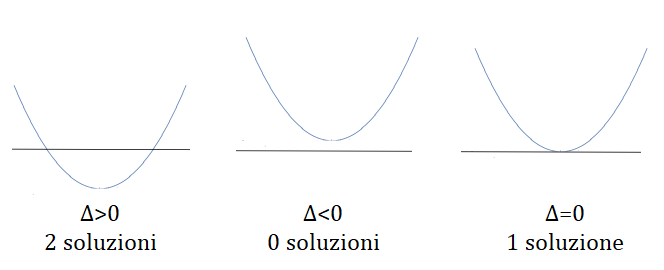
\includegraphics[width=.9\textwidth]{immagini/cap_4/fig_4_1.png}
\end{center}
\end{figure}
Pertanto
\begin{equation}
\langle i \left[R,S \right] \rangle ^2 - 4\langle R^2 \rangle \langle S^2 \rangle \leq 0,
\end{equation}
ossia
\begin{equation}
\langle R^2 \rangle \langle S^2 \rangle \geq \frac{1}{4}\langle i \left[R,S \right] \rangle ^2.
\end{equation}
Scegliendo infine $R=\Delta A$ ed $S= \Delta B$ si ottiene la relazione di indeterminazione \eqref{eq:cap4_2}.
\section[Esempio: autovalori ed autovettori dello spin per particelle di spin 1/2 e relazioni di indeterminazione]{Esempio: autovalori ed autovettori dello spin per\\ particelle di spin 1/2 e relazioni di indeterminazione}
Consideriamo nuovamente un sistema costituito da particelle di spin 1/2. Abbiamo già visto che i corrispondenti stati di singola particella possono essere espressi come combinazione lineare di sue stati di base, che qui indichiamo con $\vert +z\rangle $ e $\vert - z \rangle$, che rappresentano gli stati in cui la proiezione dello spin della particella lungo l'asse $z$ vale rispettivamente $S_z = \pm \hbar /2$. È evidente che in questa base l'operatore $S_z$ è rappresentato dalla seguente matrice:
\begin{equation}
S_z = \left( 
\begin{array}{cc}
\langle +z \vert S_z \vert +z \rangle &  \langle +z \vert S_z \vert -z \rangle \\
\langle -z \vert S_z \vert +z \rangle & \langle -z \vert S_z \vert -z \rangle  
\end{array}
\right)= \frac{\hbar}{2}\begin{pmatrix}
1 & 0 \\
0 & -1
\end{pmatrix}
\end{equation}
o, equivalentemente
\begin{equation}
S_Z =\frac{\hbar}{2}\sigma _z,
\end{equation}
dove $\sigma _z$ è la matrice di Pauli.\\
Utilizzando le proprietà generali dell'operatore di spin è possibile anche dimostrare che per gli analoghi operatori di $S_x$ ed $S_y$ valgano le corrispondenti rappresentazioni:
\begin{eqnarray}
& &\displaystyle{S_x = \frac{\hbar}{2}\sigma _x= \frac{\hbar}{2}\begin{pmatrix}
0 & 1 \\
1 & 0
\end{pmatrix}
} \\
\nonumber \\
& &\displaystyle{S_y= \frac{\hbar}{2}\sigma _y = \frac{\hbar}{2} \begin{pmatrix}
0 & -i \\
i & 0
\end{pmatrix}}
\end{eqnarray}
Poiché le tre matrici di Pauli hanno determinante uguale a $-1$ e traccia nulla, i loro autovalori sono $+1$ o $-1$. Corrispondentemente, gli autovalori della proiezione dello spin lungo un qualunque asse sono $\pm \hbar/2$. È immediato calcolare i corrispondenti autovettori:
\begin{eqnarray}
\label{eq:cap4_4}
& &\displaystyle{S_x = \frac{\hbar}{2}, \quad \vert x \rangle = \frac{1}{\sqrt{2}}\vert +z \rangle + \frac{1}{\sqrt{2}}\vert -z \rangle}= \frac{1}{\sqrt{2}}
\begin{pmatrix}
1\\
1
\end{pmatrix} \nonumber \\
\\
& &\displaystyle{S_x = -\frac{\hbar}{2}, \quad \vert -x \rangle = \frac{1}{\sqrt{2}}\vert +z \rangle - \frac{1}{\sqrt{2}}\vert -z \rangle}= \frac{1}{\sqrt{2}} \begin{pmatrix}
1\\
-1
\end{pmatrix}\nonumber
\end{eqnarray}
\begin{eqnarray}
\label{eq:cap4_5}
& &\displaystyle{S_y = \frac{\hbar}{2}, \quad \vert y \rangle = \frac{1}{\sqrt{2}}\vert +z \rangle + \frac{i}{\sqrt{2}}\vert -z \rangle}= \frac{1}{\sqrt{2}} 
\begin{pmatrix}
1\\
i
\end{pmatrix} \nonumber \\
\\
& &\displaystyle{S_y = -\frac{\hbar}{2}, \quad \vert -y \rangle = \frac{1}{\sqrt{2}}\vert +z \rangle - \frac{i}{\sqrt{2}}\vert -z \rangle}= \frac{1}{\sqrt{2}} 
\begin{pmatrix}
1\\
-i
\end{pmatrix}\nonumber
\end{eqnarray}
\begin{center}
\fbox{\begin{minipage}{.9\textwidth}
Calcoliamo esplicitamente l'autostato di $\vert +x\rangle$ di $S_x$ con autovalore $+\hbar /2$. Scriviamo questo stato come combinazione lineare generica di autostati di $S_z$:
\begin{equation}
\vert +x \rangle = c_1\vert +z \rangle+ c_2\vert -z \rangle \doteq 
\begin{pmatrix}
c_1 \\
c_2
\end{pmatrix}
\end{equation}
Applicando l'equazione agli autovalori $S_x \vert+x\rangle =\hbar /2 \vert +x\rangle $ si ottiene:
\begin{equation}
\frac{\hbar}{2}
\begin{pmatrix}
0 & 1 \\
1 & 0
\end{pmatrix}
\begin{pmatrix}
c_1 \\
c_2
\end{pmatrix} =
\frac{h}{2}
\begin{pmatrix}
c_1 \\
c_2
\end{pmatrix}
\quad \Rightarrow \quad
\begin{cases}
c_2=c_1\\
c_1=c_2
\end{cases}
\end{equation}
La condizione di normalizzazione dello stato implica:
\begin{equation}
\langle +x \vert +x \rangle = \left( c_1 ^*\ c_2 ^*\right)\begin{pmatrix}
c_1\\c_2
\end{pmatrix} = \vert c_1 \vert ^2 +\vert c_2 \vert ^2 =1, 
\end{equation}
che, unitamente alla condizione $c_1=c_2$ implica $\vert c_1 =1/\sqrt{2}$. Possiamo allora scrivere:
\begin{equation}
c_1 =c_2 = \frac{e^{i\delta}}{\sqrt{2}}\ \Rightarrow \ \vert +x \rangle \frac{e^{i\delta}}{\sqrt{2}} \left(\vert +z \rangle + \vert -z \rangle \right).
\end{equation}
Il fattore di fase moltiplicativo, nel vettore di stato, è completamente arbitrario, ossia non interviene mai nelle quantità fisiche che sono la probabilità ($\vert \langle \alpha \vert +x \rangle \vert ^2$) ed i valori di aspettazione ($\langle +x \vert A \vert +x \rangle $). Una scelta possibile è 	quella effettuata effettuata in eq. \eqref{eq:cap4_4}, ossia $e^{i\delta}=1$.
\end{minipage}}
\end{center}
È semplice verificare questi risultati. Ad esempio si ha:
\begin{equation}
S_y \vert - y \rangle = \frac{\hbar}{2\sqrt{2}}\begin{pmatrix}
0 & -i\\
i & 0
\end{pmatrix}
\begin{pmatrix}
1\\-i
\end{pmatrix} = \frac{\hbar}{2\sqrt{2}} 
\begin{pmatrix}
-1 \\ i
\end{pmatrix} = -\frac{\hbar}{2} \vert -y \rangle .
\end{equation}
Gli operatori corrispondenti alle proiezioni dello spin lungo i tre assi non commutano tra loro. Per esempio, un calcolo esplicito del commutatore di $S_x$ ed $S_y$ conduce a:
\begin{eqnarray}
\left[ S_x , S_y \right] & = & S_x S_y-S_y S_x= \nonumber \\
& = &\frac{\hbar ^2}{4} \left[\begin{pmatrix}
0 & 1\\
1 & 0
\end{pmatrix} \begin{pmatrix}
0 & -i\\
i & 0
\end{pmatrix}- \begin{pmatrix}
0 & -i\\
i & 0
\end{pmatrix}\begin{pmatrix}
0 & 1\\
1 & 0
\end{pmatrix}
\right] = \\
& = &\frac{\hbar ^2}{4} \left[\begin{pmatrix}
i & 0\\
0 & -i
\end{pmatrix} - \begin{pmatrix}
-i & 0\\
0 & i
\end{pmatrix}\right] = \nonumber \\
& = & \frac{\hbar ^2}{2}\begin{pmatrix}
i & 0\\
0 & -i
\end{pmatrix}\nonumber
\end{eqnarray}
ossia
\begin{equation}
\left[ S_x, S_y \right] = i \hbar S_z.
\end{equation}
In generale, è possibile verificare che le tre relazioni di commutazione indipendenti possono essere scritte nella forma compatta
\begin{equation}
\left[ S_i , S_j\right] = i\ \varepsilon_{ijk}\ \hbar S_k,
\end{equation}
dove gli indici 1,2,3 sono associati rispettivamente alle componenti $x$, $y$ e $z$.\\
Le relazioni di commutazione qui derivate implicano che \textbf{le componenti dello spin lungo assi distinti non possono essere misurate simultaneamente, ossia che queste tre grandezze fisiche sono osservabili incompatibili}. Corrispondentemente, deve risultare soddisfatta una \textbf{relazione di indeterminazione}. Nel caso della misura di $S_x$ ed $S_y$, per esempio, questa relazione assume la forma
\begin{equation}
\label{eq:cap4_6}
\langle (\Delta S_x) ^2 \rangle \langle (\Delta S_y) ^2 \rangle \geq \frac{1}{4} \vert \langle \left[ S_x , S_y \right] \rangle \vert ^2 = \frac{\hbar}{4} \langle S_z \rangle ^2 .
\end{equation}
Verifichiamo la validità di questa relazione per una particella che si trovi ad esempio nello stato $\vert +z\rangle$. In generale, lo scarto quadratico medio di una grandezza $A$ si esprime come
\begin{eqnarray}
\langle (\Delta A ) ^2 \rangle & = & \langle (A- \langle A \rangle ) ^2 \rangle = \langle (A^2-2A\langle A \rangle + \langle A \rangle ^2) \rangle = \nonumber \\
\\
& = & \langle A^2\rangle - \langle A \rangle ^2, \nonumber
\end{eqnarray}
e dipende dunque dai valori medi di $A$ e $A^2$.\\
Nel caso di $(\Delta S_x) ^2$, allora, calcoliamo in primo luogo l'operatore $S_x ^2$:
\begin{equation}
S_x ^2 = \frac{\hbar ^2}{4} \sigma _x ^2=\frac{\hbar ^2}{4} \begin{pmatrix}
0 & 1 \\
1 & 0
\end{pmatrix} \begin{pmatrix}
0 & 1 \\
1 & 0
\end{pmatrix} = \frac{\hbar ^2}{4}\begin{pmatrix}
1 & 0 \\
0 & 1
\end{pmatrix}.
\end{equation}
(Osserviamo che le matrici di Pauli soddisfano $\sigma _x ^2 = \sigma _y ^2 = \sigma _z ^2 =1$).\\
Poiché lo stato $\vert +z \rangle$, su cui vogliamo verifica la relazione di indeterminazione, è uno degli stati di base, i valori medi di $S_x$ ed $S_x ^2$ su questo stato si ottengono direttamente dai corrispondenti elementi di matrice (elementi 1,1):
\begin{eqnarray}
& &\displaystyle{\langle +z \vert S_x \vert +z \rangle = (S_x)_{11} = \frac{\hbar}{2}\cdot 0 =0}  \nonumber \\
\\
& &\displaystyle{\langle +z \vert S_x ^2\vert +z \rangle = (S_x ^2)_{11} = \frac{\hbar ^2}{4}\cdot 1 =\frac{\hbar ^2}{4}} \nonumber
\end{eqnarray}
Ne segue allora
\begin{equation}
\label{eq:cap4_7}
\langle +z \vert (\Delta S_x)^2\vert +z \rangle = \frac{\hbar ^2}{4}.
\end{equation}
Analogamente si calcola $\langle (\Delta S_y)^2 \rangle $ ($S_y ^2= \frac{\hbar ^2}{4}\cdot I$):
\begin{eqnarray}
& &\displaystyle{\langle +z \vert S_y \vert +z \rangle = (S_y)_{11} = \frac{\hbar}{2}\cdot 0 =0}  \nonumber \\
\\
& &\displaystyle{\langle +z \vert S_y ^2\vert +z \rangle = (S_y ^2)_{11} = \frac{\hbar ^2}{4}\cdot 1 =\frac{\hbar ^2}{4}} \nonumber
\end{eqnarray}
da cui
\begin{equation}
\label{eq:cap4_8}
\langle +z \vert (\Delta S_y)^2\vert +z \rangle = \frac{\hbar ^2}{4}.
\end{equation}
Il secondo membro della relazione di indeterminazione è in questo caso, a parte il fattore $\frac{\hbar ^2}{4}$, semplicemente il valore medio di $S_z$ al quadrato:
\begin{equation}
\label{eq:cap4_9}
\left( \langle +z \vert S_z \vert +z \rangle \right) ^2 = \frac{\hbar ^2}{4}.
\end{equation}
Mettendo insieme i risultati \eqref{eq:cap4_7}, \eqref{eq:cap4_8} e \eqref{eq:cap4_9} possiamo allora verificare esplicitamente la relazione di indeterminazione \eqref{eq:cap4_6}:
\begin{equation}
\langle  (\Delta S_x)^2 \rangle \langle(\Delta S_y)^2 \rangle = \left(\frac{\hbar ^2}{4} \right) ^2 \geq \frac{\hbar ^2}{4} \langle S_z  \rangle ^2 = \left(\frac{\hbar ^2}{4} \right) ^2.
\end{equation}
La relazione di indeterminazione risulta quindi soddisfatta, in questo caso, con il segno di uguaglianza. In altri termini, sullo stato $\vert +z \rangle $ il prodotto delle indeterminazioni su $S_x$ e $S_y$ assume il valore minimo possibile compatibilmente con la relazione di indeterminazione.\\ \\
\textbf{Appendice:}\\
Vediamo come, considerando ad esempio lo stato $\vert + z \rangle $, i valori medi $\langle S_x \rangle $ e $\langle (\Delta S_x)^2 \rangle $ possano essere calcolai anche utilizzando la definizione di valore medio:
\begin{equation}
\langle A \rangle = \sum _i a_i p_i,
\end{equation}
dove $A_I$ sono i possibili risultati della misura di $A$ e $p_i$ le corrispondenti probabilità.\\
Utilizzando le eq.\eqref{eq:cap4_7} è semplice trovare che lo stato $\vert +z \rangle$ si esprime come combinazione lineare degli autostati si $S_x$ nella forma
\begin{equation}
\vert +z \rangle = \frac{1}{\sqrt{2}} \vert +x \rangle + \frac{1}{\sqrt{2}} \vert -x \rangle .
\end{equation}
I possibili risultati di una misura di $S_x$ e le corrispondenti probabilità su questo stato sono allora
\begin{equation}
\begin{cases}
\displaystyle{S_x ^{(1)} = +\frac{\hbar}{2}, \ p_1 = \frac{1}{2}} \\
\\
\displaystyle{S_x ^{(2)} = -\frac{\hbar}{2}, \ p_2 = \frac{1}{2}}
\end{cases}
\end{equation}
Per i valori medi si $S_x$ si ottiene allora:
\begin{equation}
\langle S_x \rangle = \sum _i S_x ^{(i)} p_i= +\frac{\hbar}{2}\cdot\frac{1}{2}-\frac{\hbar}{2}\cdot\frac{1}{2}=0,
\end{equation}
mentre per lo scarto quadratico medio
\begin{equation}
\langle (\Delta S_x)^2 \rangle = \sum _i ( S_x ^{(i)}- \underbrace{\langle S_x \rangle}_{=0}) ^2\ p_i= +\frac{\hbar ^2}{4}\cdot\frac{1}{2}+\frac{\hbar ^2}{4}\cdot\frac{1}{2}= \frac{\hbar ^2}{2},
\end{equation}
in accordo con i precedenti risultati ottenuti.